\subsection{Gestione della configurazione}

% Inizio gestione della configurazione

\subsubsection{Scopo}

La gestione della configurazione definisce i principi normativi utili a predisporre il \glock{workspace} per tutto il gruppo, semplificando e automatizzando la conservazione dei documenti e delle componenti software, che andranno a formare il prodotto finale.

\subsubsection{Aspettative}

La gestione della configurazione si predispone a rendere usabile l'ambiente di lavoro, controllando attivamente e autonomamente tutte le attività in modo metodico e organizzato. Ciò è importante perché riduce la complessità di coordinamento nel corso dello sviluppo del prodotto, sia che riguardi la documentazione, sia che riguardi le componenti software.

\subsubsection{Descrizione}

Il processo di gestione della configurazione si compone di una serie di attività e strumenti atte a costituire un ambiente di lavoro semplice e ordinato. 
In particolare, si fa uso dei seguenti strumenti:
\begin{itemize}
	\item repository;
	\item tecnologie scelte.
\end{itemize}
Gli strumenti vengono utilizzati per svolgere le seguenti attività:
\begin{itemize}
	\item versionamento e rilascio del prodotto;
	\item versionamento e rilascio dei documenti;
	\item versionamento e rilascio dei componenti software;
	\item continuous integration;
	\item notification \& monitoring;
\end{itemize}


\subsubsection{Attività}

	\paragraph{Versionamento e rilascio del prodotto}

	Il prodotto viene inteso come l'insieme di componenti che dovranno essere progettate, sviluppate, verificate e validate prima di essere consegnate al cliente. Il prodotto si compone principalmente di:
	\begin{itemize}
		\item documentazione;
		\item componenti software.
	\end{itemize}

	Ciascuna componente viene versionata seguendo la propria evoluzione, mentre nel caso del prodotto si segue un versionamento più macroscopico e basato sulle \glock{baseline}.
	Nell'ambito del progetto, il gruppo ha deciso di integrare una prassi di versionamento che permetta di avere un riferimento del prodotto dalle singole componenti sviluppate.

		\subparagraph{Sintassi codice di versionamento}

		Al numero di versione di un prodotto associato ad una baseline si aggiunge il seguente identificativo:

		\[%
			\text{+b}[\alpha].[\beta]
		\]

		\begin{itemize}
			\item \((\alpha)\): numero identificativo del rilascio del prodotto
			\begin{itemize}
				\item parte da 0 e non si resetta mai;
				\item viene incrementato quando tutte le componenti sono state concluse e pronte per la consegna al cliente;
			\end{itemize}
			\item \((\beta)\): numero identificativo che viene associato a una baseline del prodotto:
			\begin{itemize}
	  			\item parte da 0 e si resetta quando \(\alpha\) viene incrementato;
				\item viene incrementato quando si raggiunge una nuova baseline di prodotto. 
			\end{itemize}
		\end{itemize}

		\subparagraph{Esempi di versionamento del prodotto}

		\begin{itemize}
			\item \textbf{v0.5.1+b0.1}: indica la versione 0.5.1 di una componente proveniente dalla baseline di prodotto in versione 0.1;
			\item \textbf{v1.13.1+b0.2}:  indica la versione 1.12.1 di una componente proveniente dalla baseline di prodotto in versione 0.2;
			\item \textbf{v3.0.2+b1.3}: indica la versione 3.0.2 di una componente proveniente dalla baseline di prodotto in versione 1.3.
		\end{itemize}

		\subparagraph{Rilascio}

		Il rilascio del prodotto viene effettuato nel momento in cui la prima cifra della versione viene incrementata. Ad essa si devono allineare tutte le altre componenti con delle versione approvate ed autorizzate per il rilascio. 

	\paragraph{Versionamento e rilascio dei documenti}

	Tutti i file che riguardano la documentazione vengono conservati in un repository e ogni documento viene versionato per mezzo di un identificativo, in base alla sua fase di avanzamento. Questo permette di poter fare riferimento alle nuove versioni del documento durante tutto il ciclo di vita del software.

		\subparagraph{Sintassi codice di versionamento}

		Ciascun documento possiede un identificativo di versionamento su ogni pagina che rispetta il seguente formalismo:

		\[%
			\text{v}[\alpha].[\beta].[\gamma]
		\]

		\begin{itemize}
			\item \((\alpha)\): numero identificativo del rilascio esterno del documento al proponente e/o al committente
				\begin{itemize}
					\item parte da 0 e non si resetta mai;
					\item viene incrementato solo dal responsabile a seguito di una approvazione di rilascio del documento verso un destinatario esterno al team;
				\end{itemize}
			\item \((\beta)\): numero identificativo che rappresenta un'approvazione del documento
				\begin{itemize}
					\item parte da 0 e si resetta solo a incrementi di \(\alpha\);
					\item viene incrementato solo dal responsabile a seguito del raggiungimento di una baseline se il prodotto è conforme;
				\end{itemize}
			\item \((\gamma)\): numero rappresentativo di una aggiunta o modifica verificata fatta al documento
				\begin{itemize}
					\item parte da 0 e si resetta solo a incrementi di \(\beta\) o di \(\alpha\);
					\item viene incrementato da un revisore dopo aver verificato che una sezione sia conforme a quanto deciso.
				\end{itemize}
		\end{itemize}

		Generalmente ogni documento prima di poter essere rilasciato verso l'esterno dovrà essere stato approvato e rilasciato internamente.

		\subparagraph{Esempi codice di versionamento dei documenti}

		\begin{itemize}
			\item \verb!v0.2.1!;
			\item \verb!v1.12.1!;
			\item \verb!v3.0.2!.
		\end{itemize}

		\subparagraph{Gestione delle modifiche}

		Le modifiche ai documenti vengono gestite seguendo il \textbf{registro delle modifiche} presente in tutti i documenti nella pagina successiva al frontespizio. All'interno di questo documento si tiene traccia di ogni aggiunta, modifica, eliminazione, revisione o approvazione da parte di tutti i membri del team. La normativa sul formalismo può essere trovata al paragrafo \ref{par: Registro modifiche} a pagina \pageref{par: Registro modifiche}.

		\subparagraph{Rilascio}

		Un documento viene rilasciato alle parti proponenti solamente quando vi è un incremento del primo numero (\(\alpha\)), che ne implica una approvazione da parte del responsabile. \\
		Per quanto concerne la distribuzione interna, tutti gli \glock{artefatti} dei documenti realizzati durante la fase di sviluppo sono resi disponibili in modo rapido e automatizzato a tutti i membri del gruppo, a cui vengono notificate tutte le modifiche tramite il \glock{workspace} di \textit{Slack}.

		\subparagraph{Integrazione con il versionamento di prodotto}

		La documentazione viene interpretata come componente, e in quanto tale riceve come aggiunta al proprio codice di versionamento anche l'identificativo di prodotto. Questo identificativo aggiuntivo viene esplicitato solamente all'interno del documento e non nella denominazione dei file.

	\paragraph{Versionamento e rilascio dei componenti software}

	I sorgenti del software che riguardano la codifica e la configurazione del prodotto da realizzare sono mantenuti nel repository, insieme alla documentazione. Ogni file viene versionato con un apposito storico delle modifiche, mentre ogni componente software viene versionato come \glock{baseline} di prodotto in relazione alle funzionalità presenti e dei requisiti obbligatori implementati.

		\subparagraph{Sintassi codice di versionamento}

		Il versionamento del software viene eseguito sulla base delle implementazioni effettuate a livello di codifica.
		In aggiunta, si definisce una sintassi di stato nella versione per definirne l'usabilità.

		\[%
			\text{v}[\delta].[\epsilon].[\mu]\text{-}[\lambda]
		\]

		\begin{itemize}
			\item \((\delta)\): numero identificativo del rilascio software per una \glock{major release}
			\begin{itemize}
				\item parte da 0 e non si resetta mai;
				\item viene incrementato solo dopo aver implementato tutti i requisiti obbligatori;
			\end{itemize}
			\item \((\epsilon)\): numero identificativo per una \glock{minor release}
			\begin{itemize}
				\item parte da 0 e si resetta solo a incrementi di \(\delta\);
				\item viene incrementato solo dopo l'implementazione di uno o più requisiti;
			\end{itemize}
			\item \((\mu)\): numero rappresentativo per una \glock{patch}
			\begin{itemize}
				\item parte da 0 e si resetta solo a incrementi di \(\epsilon\) o di \(\delta\);
				\item viene incrementato a ogni modifica di uno o più requisiti e ad ogni cambio di configurazione del software;
			\end{itemize}
			\item \((\lambda)\): sigla che identifica uno stato del software; può avere i seguenti significati in ordine crescente di stato
			\begin{itemize}
				\item \verb!dev!: derivante da \textbf{dev}elopment, versione ancora in sviluppo
					\begin{itemize}
						\item software non completo, che ha ricevuto aggiunte, modifiche o eliminazioni recenti;
						\item passa tutti i test sviluppati fino a quel momento;
						\item \textbf{non} si presta all'uso di un utente finale, poiché incompleto nelle funzionalità sviluppate;
					\end{itemize}
				\item \verb!rc!: \textbf{r}elease \textbf{c}andidate, versione candidata al rilascio
				\begin{itemize}
					\item software che contiene tutti o una parte dei requisiti obbligatori richiesti;
					\item passa tutte le tipologie di test;
					\item si presta all'uso di un utente finale;
				\end{itemize}
				\item \verb!stable!: versione \textbf{stabile}, pronta al rilascio pubblico
				\begin{itemize}
					\item software completo che implementa tutti i requisiti obbligatori;
					\item passa tutte le tipologie di test ed è validato;
					\item può essere collaudato con il proponente e/o pubblicato.
				\end{itemize}
			\end{itemize}
		\end{itemize}

		Una versione del software subisce un incremento di stato in base alla sua completezza in termini di funzionalità e requisiti soddisfatti. In particolare:
		\begin{itemize}
			\item una versione può ricevere lo stato di \verb!rc! solo se il primo numero (\(\delta\)) o il secondo numero (\(\epsilon\)) è diverso da 0;
			\item una versione può ricevere lo stato di \verb!stable! solo se il primo numero (\(\delta\)) è diverso da 0.
		\end{itemize}

		\subparagraph{Esempi codice di versionamento}

		\begin{itemize}
			\item \verb!v0.3.5-dev! : versione non completa, non usabile e in parte funzionante;
			\item \verb!v0.7.0-rc! : versione non completa, usabile, funzionante e con alcuni requisiti implementati;
			\item \verb!v1.0.0-rc! : versione completa, usabile, funzionante, verificata e validata;
			\item \verb!v1.0.0-stable! : versione completa, usabile, funzionante, verificata e validata, pronta al rilascio o al collaudo.
		\end{itemize}

		\subparagraph{Rilascio}

		Le release del software vengono eseguite internamente nel \glock{repository} in base alle funzionalità sviluppate. Inoltre, i rilasci interni saranno normati come segue:
		\begin{itemize}
			\item le versioni \verb!stable! e/o \glock{Major Release} devono essere approvate dall'\glock{amministratore} e dal \glock{responsabile};
			\item le versioni \verb!rc! e/o \glock{Minor Release} devono essere approvate, previa notifica di conferma di tutti i \glock{test}, dall'\glock{amministratore} e dai \glock{verificatori};
			\item le versioni \verb!dev! e/o \glock{Patch} non richiedono approvazione e possono essere rilasciate autonomamente dal programmatore.
		\end{itemize}

		\subparagraph{Integrazione con il versionamento di prodotto}

		Il software, che è formato da diverse parti con le proprie evoluzioni, viene considerato come componente del prodotto. Pertanto, nel codice di versionamento viene aggiunto in coda l'identificativo della baseline di prodotto su cui si basa. Questa prassi non si applica alla nomenclatura dei nomi dei file che riportano la versione.

	\paragraph{Continuous Integration}

	L'attività di \textit{Continuous Integration} viene praticata per eseguire degli incrementi a livello di funzionalità delle componenti del prodotto. In particolare, permette di controllare l'aggiunta e la rimozione di parti di codice con i test che vengono appositamente creati.

	La \textit{Continuous Integration} permette quindi di lavorare in modo sufficientemente sicuro, così da avere a disposizione un prodotto sempre funzionante che viene costruito a piccoli pezzi, i cui errori possono essere facilmente identificati e revisionati da parte dei programmatori e dei verificatori.

		\subparagraph{Github Actions}

		Nell'ambito del progetto, si fa uso delle \glock{Github Actions} per eseguire l'attività di integrazione continua. Una \textit{action} è un insieme di uno o più operazioni (\textit{job}) che devono essere eseguiti su una istanza virtuale di un sistema operativo. È importante fare riferimento a quanto segue:

		\begin{itemize}
			\item una singola operazione, per considerarsi corretta, deve avere un codice di uscita (\textit{exit code}) positivo (0);
			\item il fallimento di una \glock{Github Actions} può avvenire nel momento in cui il processo venga manualmente annullato, oppure una operazione ha avuto un codice di uscita negativo (1);
			\item una operazione può essere eseguita sulla istanza corrente del sistema operativo selezionato dalla configurazione corrente;
			\item gran parte delle operazioni vengono eseguite su \glock{Docker} in contenitori indipendenti e su nuove istanze appositamente generate;
			\item una \textit{action} può essere avviata sul repository ospitante.
		\end{itemize}

		La struttura sequenziale delle operazioni è la seguente:

		\begin{itemize}
			\item configurazione delle operazioni da eseguire;
			\item esecuzione delle operazioni con riscontro dei codici di uscita;
			\item esito finale e notifica sui canali telematici agli attori interessati.
		\end{itemize}

		\subparagraph{Documentazione}

		Il repository è stata configurata per garantire una buona accessibilità e correttezza nello sviluppo dei documenti di progetto da parte dei membri del team. A tal proposito, è stato messo in atto un processo di integrazione continua in ambiente di sviluppo nel momento in cui si vuole eseguire un incremento di versione di un documento. 
		Seguendo la configurazione del workflow adottata per il progetto, a partire da una modifica di un documento che viene eseguito su un branch \verb!feature/!, il documento deve essere sempre compilabile in \LaTeX{}. 
		Viene quindi eseguito un controllo preventivo prima di permettere l'integrazione finale delle modifiche tali da essere convalidate.

		\begin{enumerate}
			\item ad ogni \textit{pull request} da un branch \verb!feature! al \verb!develop!, viene eseguita una \glock{build} di controllo di tutti i documenti modificati;
			\item se è tutto corretto, la \glock{build} crea un \glock{artefatto} con tutti i documenti PDF, che viene salvato nel repository e reso disponibile per essere visionato da remoto:
			\begin{itemize}
				\item \href{https://artifacts.redroundrobin.site}{artifacts.redroundrobin.site}
			\end{itemize}
			\item tramite gli appositi canali di comunicazione, vengono notificati tutti i membri del team delle nuove modifiche ai documenti.
		\end{enumerate}

		Nel caso di \textbf{errori} nella compilazione dei file, viene inviato un avviso all'ultima persona che ha eseguito il \glock{commit} e vengono mantenuti gli ultimi file correttamente compilati.

		\subparagraph{Componenti software}

		I singoli componenti fanno uso delle \glock{Github Actions} per l'attività di integrazione continua. In particolare, in base alla tipologia di componente, vengono create delle operazioni di controllo basate sui \glock{Test} per verificare i requisiti del progetto.
	

	\paragraph{Notification \& monitoring}

	L'attività di \textit{notification \& monitoring} permette di notificare i membri del team al fine di avere sempre sotto controllo le modifiche effettuate in un componente del prodotto. Questo, ad esempio, permette di venire a conoscenza dei fallimenti o successi per l'attività di \textit{Continuous Integration}. In questo caso, notifiche più specifiche possono essere inviate solamente ai membri interessati che sono stati coinvolti nel processo di modifica della componente. 
	\newline
	Generalmente, si usano i seguenti canali telematici per le notifiche:
	\begin{itemize}
		\item pagina delle GitHub Actions del repository;
		\item email automatiche;
		\item canali Slack.
	\end{itemize}

	Il \textbf{monitoraggio} viene eseguito principalmente per mezzo di notifiche. Tuttavia, poiché il coordinamento risulta essere di essenziale importanza, si è deciso di integrare uno strumento che traccia in tempo reale gli ultimi avvenimenti all'interno di un repository da parte dei singoli membri del gruppo.
	Questo strumento, denominato \textit{Workflow Tracker}, permette di individuare l'ultimo branch in cui un utente ha lavorato, così da ridurre preventivamente i conflitti delle modifiche e sapere le ultime attività all'interno del repository.
	\newline
	Lo strumento è pubblicamente visibile e reperibile al seguente indirizzo per tutti i membri del gruppo:
	\begin{itemize}
		\item \href{https://workflow.redroundrobin.site}{workflow.redroundrobin.site}
	\end{itemize}
	Il \textit{workflow tracker} aggiorna automaticamente ogni 20 secondi gli ultimi movimenti all'interno di una repository e identifica tutti gli autori che hanno eseguito un'azione di \textit{push} all'interno del repository.



\subsubsection{Metriche}

La gestione della configurazione non fa uso di particolari metriche per misurare la qualità.


\subsubsection{Strumenti}

	\paragraph{Repository}
	
	Il repository è un luogo remoto in cui vengono mantenuti, salvati e versionati tutti i file che riguardano il progetto per tutto il ciclo di vita del prodotto.
	\newline
	Questo risiede in modo condiviso all'interno di \glock{GitHub} ed è accessibile solamente ai membri del team.

		\subparagraph{Versionamento con GitHub}

		Il repository fa uso di un \textit{Version Control System} (VCS) di tipo distribuito sotto il motore \textit{Git}, che permette la condivisione dal locale al remoto del proprio spazio di lavoro su un luogo comune.
		\newline
		Attraverso l'utilizzo di un web browser, è possibile collegarsi a \textit{GitHub} e controllare i file contenuti in un repository. 

		\subparagraph{Configurazione del workflow}

		Usando \textit{Git}, è possibile clonare e scaricare da remoto tutto il contenuto del repository per averne una copia in locale su cui poter lavorare, visionando la cronologia dei file modificati ad ogni \glock{commit} da parte di un membro del gruppo.
		\newline
		\textit{Git}, inoltre, include la possibilità di creare dei \glock{branch} (locali e remoti) in cui poter sviluppare in maniera indipendente una funzionalità, che potrà essere integrata successivamente, senza bisogno di stare al passo con gli aggiornamenti del repository.

		Pertanto, si è deciso di stabilire il seguente canone di \glock{workflow} per quanto concerne la documentazione:
		\begin{itemize}
			\item \verb!master! branch: branch principale su cui vengono fatti i rilasci ad ogni \glock{milestone};
			\item \verb!develop! branch: branch di sviluppo su cui viene fatta integrazione di nuove funzionalità concluse;
			\item \verb!feature/xxxx! branch: branch indipendente usato da uno o più membri del gruppo per sviluppare una sezione o fare una revisione di un documento;
			\begin{itemize}
				\item \textbf{xxxx:} si riferisce al numero della \glock{issue} o al titolo della funzionalità da integrare.
				\item il \textit{feature branch} riferisce generalmente una singola \glock{issue} ed è rimosso alla sua chiusura.
			\end{itemize}
		\end{itemize}

		Ad ogni milestone viene associata una release interna al repository, così da tenere traccia di una \glock{baseline}.

		\subparagraph{Cartelle di configurazione}

		Il repository si compone di diverse tipologie di cartelle. Oltre alle cartelle che riguardano la documentazione e il software, è presente una cartella che viene usata ai fini della configurazione di \glock{GitHub}.
		\begin{itemize}
			\item \verb!.github/!: cartella per il repository di \glock{Github} con i file di configurazione per le \glock{Github Actions} e l'\glock{Issue Tracking System}.
		\end{itemize}

		\subparagraph{Formati dei file per le configurazione}

		In generale, vengono utilizzati alcuni file con formati speciali per la configurazione del repository. Questi file vanno modificati solamente dall'\glock{amministratore}, o su richiesta, anche da parte di altri membri del gruppo, in base alle necessità.
		\begin{itemize}
			\item \textbf{.gitignore} contiene tutte le regole per evitare di caricare nel repository dei formati non autorizzati (es: file eseguibili);
			\item \textbf{.yml} contiene la configurazione di una \glock{GitHub Action} per dirigere il \glock{Workflow};
			\item \textbf{file senza formati} contengono configurazioni aggiuntive per \glock{GitHub} (es: template delle \glock{Issue});
		\end{itemize}

		\subparagraph{Formati dei file per i documenti}

		Per la documentazione si usano principalmente i seguenti tipi di file:
		\begin{itemize}
			\item \textbf{file .tex:} contiene il codice sorgente \LaTeX{} del documento;
			\item \textbf{file .pdf:} è il documento compilato;
			\item \textbf{file .png:} identifica una immagine;
			\item \textbf{file .md:} identifica un file scritto in \glock{Markdown}, generalmente usato per gli appunti.
		\end{itemize}


	\paragraph{Project board}

	Al fine di ottenere un coordinamento il più possibile trasparente dei compiti di un singolo membro del gruppo, si è deciso di introdurre, attraverso la suite di \glock{Github}, una \textbf{project board} generale che permette di visionare l'andamento dei task, dalla loro creazione fino al loro completamento.
	\newline
	La project board può essere acceduta e visionata solamente dai membri del team al seguente indirizzo:

	\href{http://project.redroundrobin.site}{http://project.redroundrobin.site}

		\subparagraph{Issue tracking system}

		\textit{GitHub} integra un \textit{Issue Tracking System} (ITS) che permette di tracciare lo sviluppo tramite ticketing, assegnando a ciascun membro del team una o più \glock{issue} in base alle necessità.
		\newline
		L'ITS viene attivato su ogni repository di progetto e ciascuno viene poi collegato nella project board generale.
		\newline
		Una \glock{issue} descrive un problema che deve essere risolto, sia riguardante l'introduzione di una nuova funzionalità, sia per la risoluzione di un bug. Inoltre, una qualunque \glock{issue} può essere:
		\begin{itemize}
			\item assegnata a uno o più membri del team;
			\item aperta o chiusa;
			\item assegnata a una milestone;
			\item assegnata a una project board;
			\item discussa a mo' di \textit{forum} da tutti i membri del gruppo.
		\end{itemize}


	\paragraph{Git submodules}

	Analizzando il quantitativo di componenti software, sono stati individuati dei possibili problemi che potrebbero sorgere qualora si decidesse di mantenere tutte le componenti del prodotto in un solo luogo.
	\newline
	Un grande quantitativo di cartelle può causare confusione e rallentamento nello sviluppo, specialmente nel momento in cui si rende necessario \textbf{collaborare} tramite i branch.
	\newline
	Decidendo di lavorare con un workflow basato sui \textit{feature branch}, il fatto di lavorare su più componenti può portare a un \textbf{livello di astrazione maggiore}, che può comportare problemi di coordinamento e conflitti nelle componenti realizzate.

		\subparagraph{Introduzione ai sotto-moduli}

		Al fine di porre rimedio a questa eventuale problematica, si è deciso di introdurre una funzionalità di \glock{Git} per poter separare lo sviluppo delle componenti software in più \textbf{sotto-moduli}.
		\newline
		Ciascun sotto-modulo viene identificato come un repository indipendente, dove viene sviluppata una componente software seguendo la stessa configurazione di \textit{workflow}.
		\newline
		Tutti i sotto-moduli possono essere singolarmente recuperati e versionati in un repository principale, in cui si va a comporre l'intero prodotto seguendo l'andamento di rilascio delle relative \textit{baseline} di prodotto.

		\begin{itemize}
			\item un sotto-modulo si identifica come repository di \glock{github};
			\item un sotto-modulo può essere aggiornato nel repository principale seguendo gli ultimi commit nel branch principale o recuperando la versione di rilascio;
			\item nel repository principale, solo l'amministratore aggiorna manualmente le versioni dei componenti (o sotto-moduli) in base ai rilasci di prodotto.
		\end{itemize}

		\subparagraph{Repository principale}

		Il repository principale si compone di tutti i sotto-moduli che vengono versionati in base all'ultimo commit nel sotto-modulo o in base alla versione rilasciata del sotto-modulo.
		\newline
		La struttura di dipendenza dei repository è la seguente:

		\begin{itemize}
			\item \verb!swe-thirema!: repository principale con il prodotto intero
			\begin{itemize}
				\item \verb!swe-docs!: sotto-modulo per la documentazione;
				\item \verb!swe-webapp!: sotto-modulo per il sito web di progetto;
				\item \verb!swe-api!: sotto-modulo per le \glock{API};
				\item \verb!swe-telegram!: sotto-modulo per il \glock{Bot Telegram};
				\item \verb!swe-kafka-db!: sotto-modulo per i database e \glock{Apache Kafka};
				\item \verb!swe-gateway!: sotto-modulo per il \glock{Gateway} e i dispositivi.
			\end{itemize}
		\end{itemize}

		\begin{figure}[H]
			\centering
			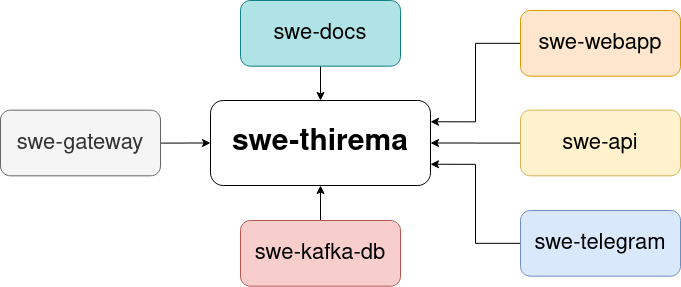
\includegraphics[scale=0.7]{res/images/submodules}
			\caption{Grafico riassuntivo dei Git submodules utilizzati nel progetto}
		\end{figure}
		
		Il repository principale può essere acceduta dal seguente indirizzo:

		\href{https://github.com/RedRoundRobin/swe-thirema}{thirema.redroundrobin.site}

		\subparagraph{Sotto-modulo swe-docs}

		\begin{itemize}
		 	\item \textbf{descrizione:} contiene tutta la documentazione di progetto;
		 	\item \textbf{nome completo:} \verb!RedRoundRobin/swe-docs!;
		 	\item \textbf{URL:} \href{https://github.com/RedRoundRobin/swe-docs}{docs.redroundrobin.site};
		 	\item \textbf{linguaggi di sviluppo:} \LaTeX{};
		 	\item \textbf{struttura delle cartelle:}
			\begin{itemize}
				\item \verb!interni/!: contiene tutta la documentazione interna;
				\item \verb!esterni/!: contiene tutta la documentazione esterna;
				\item \verb!template/!: contiene tutti i template delle varie tipologie di documento;
				\item \verb!notes/!: contiene tutte le note aggiuntive (\textit{non}-\LaTeX{}) sui seminari, le guide e l'organizzazione.
			\end{itemize}
		 \end{itemize}

		\subparagraph{Sotto-modulo swe-webapp}

		\begin{itemize}
		 	\item \textbf{descrizione:} contiene il sito web richiesto dal progetto;
		 	\item \textbf{nome completo:} \verb!RedRoundRobin/swe-webapp!;
		 	\item \textbf{URL:} \href{https://github.com/RedRoundRobin/swe-webapp}{webapp.redroundrobin.site};
		 	\item \textbf{linguaggi di sviluppo:} \glock{PHP}, \glock{Javascript}.
		 \end{itemize}

		\subparagraph{Sotto-modulo swe-api}

		\begin{itemize}
		 	\item \textbf{descrizione:} contiene le \glock{API} per la comunicazione tra \glock{Apache Kafka} e le applicazioni esterne;
		 	\item \textbf{nome completo:} \verb!RedRoundRobin/swe-api!;
		 	\item \textbf{URL:} \href{https://github.com/RedRoundRobin/swe-api}{api.redroundrobin.site};
		 	\item \textbf{linguaggi di sviluppo:} \glock{Java}.
		 \end{itemize}

		\subparagraph{Sotto-modulo swe-telegram}

		\begin{itemize}
		 	\item \textbf{descrizione:} contiene il \glock{Bot Telegram};
		 	\item \textbf{nome completo:} \verb!RedRoundRobin/swe-telegram!;
		 	\item \textbf{URL:} \href{https://github.com/RedRoundRobin/swe-telegram}{telegram.redroundrobin.site};
		 	\item \textbf{linguaggi di sviluppo:} \glock{Javascript}.
		 \end{itemize}

		\subparagraph{Sotto-modulo swe-kafka-db}

		\begin{itemize}
		 	\item \textbf{descrizione:} contiene il componente per la configurazione di \glock{Kafka} e dei database;
		 	\item \textbf{nome completo:} \verb!RedRoundRobin/swe-kafka-db!;
		 	\item \textbf{URL:} \href{https://github.com/RedRoundRobin/swe-kafka-db}{kafka-db.redroundrobin.site};
		 	\item \textbf{linguaggi di sviluppo:} \glock{SQL}.
		 \end{itemize}

		 \subparagraph{Sotto-modulo swe-gateway}

		\begin{itemize}
		 	\item \textbf{descrizione:} contiene l'implementazione di un \glock{Gateway} con l'integrazione di un dispositivo;
		 	\item \textbf{nome completo:} \verb!RedRoundRobin/swe-gateway!;
		 	\item \textbf{URL:} \href{https://github.com/RedRoundRobin/swe-gateway}{gateway.redroundrobin.site};
		 	\item \textbf{linguaggi di sviluppo:} \glock{Java}.
		 \end{itemize}


	\paragraph{Tecnologie di supporto e software}

	Le tecnologie e i software coinvolti per la configurazione del workflow si pongono i seguenti obiettivi:
	\begin{itemize}
		\item uniformare il \textit{modus operandi} del gruppo, consentendo di collaborare su programmi comuni e multi-piattaforma;
		\item automatizzare il lavoro per delegare gli impieghi che possono essere svolti tramite macchina, velocizzando lo sviluppo.
	\end{itemize}

		\subparagraph{Programmi per la gestione del repository}

		Il repository viene gestita principalmente in un server remoto, accessibile tramite il portale di \href{https://github.com}{Github.com} da tutti i membri del team.
		\newline
		Il processo di sviluppo, tuttavia, avviene in locale, eseguendo una clonazione del repository con tutti i branch attivi tramite uno dei seguenti programmi:
		\begin{itemize}
			\item \textbf{Github Desktop:} applicazione ufficiale di Github, molto semplice e leggera, disponibile per Linux, Mac OS e Windows;
			\item \textbf{GitKraken:} applicazione compatibile e più avanzata di Github desktop, disponibile per tutte le piattaforme;
			\item \textbf{Git CLI:} applicazione da terminale, disponibile per tutte le piattaforme con tutti i comandi utili per Git.
		\end{itemize}
		Per ciascun programma viene richiesta autenticazione, che può avvenire tramite semplice login (username e password) o tramite generazione di chiavi SSH, successivamente importate tramite una procedura guidata su \glock{Github}.

		\subparagraph{Automazione del workflow}

		Il repository, che fa uso di \glock{Github}, integra nativamente uno strumento denominato \glock{Github Actions} che permette di configurare le seguenti attività:
		\begin{itemize}
			\item \textbf{Continuous Integration:} integrazione continua del software con controllo sui \glock{Test};
			\item \textbf{Continuous Delivery:} consegna continua del software sfruttando gli incrementi minori per eseguire test più spesso;
			\item \textbf{Continuous Deployment:} distribuzione continua e messa in funzione del software;
			\item \textbf{notification \& monitoring:} invio di notifiche ai membri del team e monitoraggio delle attività di \glock{DevOps}.
		\end{itemize}
		Nel nostro caso, le \glock{Github Actions} permettono di fare in un solo file di configurazione tutti i passaggi in base al \glock{workflow} che ci interessa integrare. 
		\newline
		Delle operazioni descritte precedentemente, si fa uso solamente di:
		\begin{itemize}
			\item Countinuous Integration;
			\item notification \& monitoring.
		\end{itemize}
		I rimanenti processi verranno eventualmente impiegati per la manutenzione del prodotto.


	\paragraph{Automazione delle build e delle dipendenze}

	Per ciascun componente software, si è deciso di integrare degli strumenti di building automation col fine di semplificare la gestione delle dipendenze e l'avvio dei processi di automazione attraverso le \glock{Github Actions}.
	\newline
	In particolare, si è deciso di utilizzare:
	\begin{itemize}
		\item \verb!maven:! utilizzato in ambiente Java, molto conosciuto e facilmente integrabile;
		\item \verb!npm:! \textit{node package manager}, usato in ambiente Javascript;
		\item \verb!composer:! usato in ambiente PHP, integrato con il framework \textit{Laravel}.
	\end{itemize}

	Tutti questi strumenti sono stati configurati, rispettivamente, all'interno di ciascuna componente software che ne fa uso, con delle regole per l'analisi statica, versioni dei pacchetti da utilizzare e suite test di default da eseguire.	

	\begin{center}
		\rowcolors{2}{lightest-grayest}{white}
		\begin{longtable}{|c|c|c|c|}
		\hline
		\rowcolor{lighter-grayer}
		 & \textbf{maven} & \textbf{npm} & \textbf{composer} \\
		\hline
		\endfirsthead
		swe-docs & & &  \\ \hline
		swe-webapp & & \checkmark & \checkmark  \\ \hline
		swe-api & \checkmark & &  \\ \hline
		swe-telegram & & \checkmark &  \\ \hline
		swe-kafka-db & \checkmark & &  \\ \hline
		swe-gateway & \checkmark & &  \\
		\hline
		\caption{Tabella riassuntiva dei componenti software che fanno uso degli strumenti di building automation e gestione delle dipendenze.}
		\end{longtable}
	\end{center}

		\subparagraph{Maven} 	

		Maven è uno strumento sviluppato da \textit{Apache} e utilizzato per la gestione del progetto, esso permette di configurare tutte le dipendenze e tutti i plugin utili allo sviluppo di una applicazione \textit{Java}.
		\newline
		Integrato con \textit{IntelliJ Idea}, permette di configurare automaticamente il repository di progetto, scaricando e cancellando autonomamente le dipendenze necessarie, in base a quanto riportato nel \verb!pom.xml!.
		\newline
		Questo file si trova nella cartella principale del \textit{git submodule} in cui viene sviluppata l'applicazione \textit{Java} e può essere modificato in base alle necessità. Di seguito si mostra un esempio di \verb!pom.xml!:

		\begin{lstlisting}[language=xml,captionpos=b,caption={Esempio di implementazione di un file pom.xml}]
			<?xml version="1.0" encoding="UTF-8"?>
			<project xmlns="http://maven.apache.org/POM/4.0.0"
			         xmlns:xsi="http://www.w3.org/2001/XMLSchema-instance"
			         xsi:schemaLocation="http://maven.apache.org/POM/4.0.0 http://maven.apache.org/xsd/maven-4.0.0.xsd">
			    <modelVersion>4.0.0</modelVersion>
			
			    <groupId>groupId</groupId>
			    <artifactId>swe-gateway</artifactId>
			    <version>1.0-SNAPSHOT</version>
			    
			    <dependencies>
			        <dependency>
			            <groupId>org.apache.kafka</groupId>
			            <artifactId>kafka_2.13</artifactId>
			            <version>2.4.0</version>
			        </dependency>
			        
			        <dependency>
			            <groupId>org.jetbrains</groupId>
			            <artifactId>annotations-java5</artifactId>
			            <version>RELEASE</version>
			            <scope>compile</scope>
			        </dependency>
			
			        <!-- ... -->
			    </dependencies>
			    
			    <build>
			        <plugins>
			            <plugin>
			                <groupId>org.apache.maven.plugins</groupId>
			                <artifactId>maven-compiler-plugin</artifactId>
			                <version>3.8.0</version>
			                <configuration>
			                    <release>11</release>
			                </configuration>
			            </plugin>
			        </plugins>
			    </build>
			</project>
		\end{lstlisting}

		\subparagraph{npm - Node Package Manager}

		\textit{Node Package Manager} viene utilizzato in ambiente Javascript per la gestione delle dipendenze.
		\newline
		Il suo punto di forza risulta essere la gestione delle componenti, le quali possono essere salvate all'interno di un file \textit{json}, denominato \textit{package.json}.
		\newline
		Questo file viene utilizzato per salvare la configurazione di tutti i moduli che si vogliono integrare nel proprio progetto e che devono essere compilati a corredo del prodotto.
		\newline
		Per ciascun modulo vengono risolte poi le dipendenze attraverso un nuovo file denominato \textit{package-lock.json}, che viene versionato assieme al \textit{package.json}. In aggiunta:
		\begin{itemize}
			\item le installazioni e le rimozioni di moduli possono essere fatte tramite \textbf{npm-cli}, il programma ufficiale di npm a riga di comando;
			\item ogni volta che si esegue un aggiornamento delle dipendenze, vengono mostrate le ultime vulnerabilità scoperte con le relative correzioni;
			\item la compatibilità è assicurata su qualsiasi sistema operativo e soprattutto con gli IDE usati nel progetto;
			\item la cartella \verb!node_modules/! che viene generata alla prima configurazione di \textit{npm} \textbf{non} deve essere versionata.
		\end{itemize}

		\subparagraph{Composer}

		\textit{Composer} viene utilizzato come gestore delle dipendenze in ambiente PHP.
		\newline
		Associato al framework \glock{Laravel}, permette di integrare, in modo affine a \textit{npm}, le stesse funzionalità.
		\newline
		Infatti, viene utilizzata una interfaccia a riga di comando, da cui eseguire tutte le operazioni di installazione, aggiornamento e rimozione dei moduli usati; si ritrova, anche in questo caso, le notifiche di vulnerabilità delle dipendenze installate.
		\newline
		\textit{Composer} utilizza un file \textit{composer.json} che contiene tutti i componenti che vengono utilizzati a corredo dell'applicazione. In aggiunta:
		\begin{itemize}
			\item le installazioni e le rimozioni di moduli possono essere fatte a riga di comando tramite il comando \verb!composer!;
			\item la compatibilità è assicurata su qualsiasi sistema operativo e soprattutto con gli IDE usati nel progetto;
			\item la cartella \verb!vendor/! che viene generata alla prima configurazione di \textit{composer} \textbf{non} deve essere versionata.
		\end{itemize}


	\paragraph{Strumenti video}

	Al fine di eseguire registrazioni di video dimostrativi, sono stati utilizzati degli strumenti per la registrazione dello schermo e per il montaggio finale. In particolare, si è fatto uso di strumenti gratuiti e con molteplice compatibilità a livello di sistema operativo.

		\subparagraph{OBS}

		Il software OBS è stato utilizzato per eseguire le registrazione dei contenuti del video.
		\newline
		Il software è molto semplice e intuitivo da usare dal momento che è possibile avviare la registrazione di una sorgente (monitor) o di un'unica porzione di schermo.
		\newline
		Il video registrato può essere poi salvato con formati differenti, tipicamente \verb!.mp4!, ed esportato su una cartella di destinazione. 

		\subparagraph{DaVinci Resolve}

		Il software DaVinci Resolve è uno strumento di editing e montaggio video con diversi livelli di complessità.
		\newline
		Nell'ambito del progetto, si rende sufficiente utilizzare la modalità \textit{Cut} che permette l'aggregazione delle clip audio e video in modo del tutto intuitivo.
		\newline
		Le operazioni basilari che si possono svolgere in questa modalità riguardano:
		\begin{itemize}
			\item l'aggregazione di più clip video in modo sequenziale;
			\item l'aggiunta di più tracce audio, anche sovrapposte;
			\item il ritaglio delle clip video e audio;
			\item l'inserimento di transizioni tra più clip video.
		\end{itemize}
		Il video, una volta completato, viene poi esportato in formato \verb!.mp4! o in un formato differente in base alle esigenze.

		\subparagraph{YouTube}

		YouTube è una piattaforma online di pubblicazione e streaming video che si integra nativamente con un account Google. L'inserimento dei video è gratuito e il suo utilizzo è molto intuitivo.
		\newline
		Attraverso l'uso dell'account Google di progetto, si è deciso di aprire un canale YouTube in forma privata col fine di pubblicare video in base alle necessità.
		\newline
		I video pubblicati all'interno del canale di progetto sono solamente in forma privata e accessibili unicamente tramite link.
  

